%
% Formato padrão de slide 4x3, caso queria 16x9 remova o comentário do aspectratio
% Lembre que muitos projetores são 4x3
% se for alterar o formato é importante revisar se todos frames ficaram bons
%
\documentclass[%
    %final, % com final os TODOs (todonotes) não são apresentados
    %aspectratio=169,
    english,
    brazil]{ifsp-spo-beamer}

% um exemplo de configuração para deixar os links com cor diferenciada...
\hypersetup{breaklinks=true,colorlinks=true, linkcolor=, urlcolor=blue, citecolor=blue}

%
%
% Utilizando documento e apresentação no mesmo projeto no overleat é necessário fazer recompilação completa
%
\usepackage{longtable}
\usepackage{lscape}
\usepackage{pdflscape}

\title[Metaverso]{Metaverso - Ferramenta de Chamados de TI (ITSM) para pessoas físicas e pequenas empresas}
\subtitle{}
\date{}
\AtBeginDocument{%
% Para multiplos autores em formato tabular a lista definição deve ficar dentro do bloco do documento    
% https://tex.stackexchange.com/questions/223042/align-the-author-names-in-handout-of-beamer-by-tabular-environment
% Uma possibilidade para a lista de autores resumida que aparece no rodapé é utilizar as iniciais dos participantes
\author[ Grupo 2]{%
    \begin{tabular}{lr}
        %CEZAR GODOY NASCIMENTO & SP3040755 \\
        HENRIQUE HIROMI SHIMADA & SP3039421 \\
        ISABELA SOUZA DUARTE & SP3030083 \\
        MATEUS SOUZA DA SILVA & SP3022374 \\
        VINICIUS GOMES MOREIRA & SP3039587 \\
        WELEN MOTA SOUSA & SP146616X \\
    \end{tabular}}
}

% \subject{\inserttitle - \insertsubtitle} % metadata - titulo do PDF



% uma técnica que pode ser utilizada para facilitar o gerenciamento de quem fala durante a apresentação é redefinir os autores para que no rodapé sejam apresentados de forma diferente
%\author[\textit{Autor1} | Autor2]{.....}
%\author[Autor1 | \textit{Autor2}]{.....}


\begin{document}


\begin{frame}
  \titlepage
\end{frame}

\begin{frame}{Agenda}
 \begin{multicols}{2}
      \tableofcontents
 \end{multicols}
\end{frame}



\section[Introdução]{Introdução}

\begin{frame}{Introdução} 
\begin{itemize}
  \item 80,2\% dos domicílios brasileiro têm acesso à internet, mas a maioria desses acessa apenas via celular;

  \item As diferenças de interfaces de usuário (UI) podem ser um desafio para pessoas que transicionam de dispositivos no desenvolvimento das tarefas do dia a dia, passando desde dispositivos móveis até desktops;

  \item Fóruns são uma fonte rica de informação, mas as pessoas não estão dispostas ou não se sentem capazes de resolver seus problemas do dia a dia com as informações disponíveis.
  
\end{itemize}
\end{frame}

\section{Problema}

\begin{frame}{Problema} 
\begin{itemize}
  \item Identificamos a carência de uma alternativa para solucionar situações do cotidiano do usuário comum através uma interface que propõe soluções fáceis, mas também presta suporte similar ao corporativo para casos em que a solução não seja alcançada.
\end{itemize}
\end{frame}

\section{Objetivos}

\begin{frame}{Objetivos} 
    \begin{itemize}
			
		\item
		Familiarizar o usuário com pouca habilidade para resolver problemas de soluções simples com computadores pra que possam ser independentes;
		
		\item
		Facilitar a identificação e aplicação de resolução a problemas com computadores;
		
		\item
		Orientar os gestores da ferramenta sobre as questões e dificuldades mais comuns;
		
		\item 
		Facilitar o processo de resolução em caso de atendimento por terceiro credenciado
		
	\end{itemize}
\end{frame}

\section{Análise de Mercado}

    \begin{frame}{Análise de mercado}
    
        \begin{table} \centering
            \begin{figure}
                    \centering
                	\caption{\label{analise}Comparativo de concorrência}
                	\includegraphics[width=0.8\textwidth]{image/analise-comparativa.JPG}
                    \fonte{Os autores}
            \end{figure}
        \end{table}
    \end{frame}
    
\section{Organização da Equipe}

    \begin{frame}{Organização da Equipe}
        \begin{table} \centering
            \begin{figure}
                \centering
            	\caption{\label{analise}Organização da Equipe}\resize
            	\begin{table}[]
            	    \resizebox {.75 \textwidth }{!}{
                    \begin{tabular}{|l|l|l|l|l|l|}
                        \hline
                        Tarefa         			 & Henrique & Isabela & Mateus & Vinicius & Welen \\ \hline
						Front-End                &		&	X	&	X	&	X	&		\\ \hline
						Back-End                 &	X	&		&		&		&		\\ \hline
						Banco de Dados           &	X	&		&		&	X	&		\\ \hline
						Documentação e Modelagem &	X	&	X	&	X	&		&		\\ \hline
						Vídeos                   &	X	&	X	&	X	&	X	&	X	\\ \hline
						Blog                     &	X	&	X	&	X	&	X	&	X	\\ \hline
                    \end{tabular}
                    }
                \end{table}
                \fonte{Os autores}
            \end{figure}
        \end{table}
    \end{frame}


\section{Arquitetura da Solução}

\begin{frame}{Diagrama de Arquitetura da Solução}
    \begin{table} \centering
        \begin{figure}
                \centering
            	\caption{\label{analise}Diagrama de Arquitetura da Solução}
            	
\includegraphics[width=0.8\textwidth]{image/arquitetura_v1.png}
                \fonte{Os Autores}
        \end{figure}
    \end{table}
\end{frame}

\section{Tecnologias}
%Opção por plataformas com licenças livres para desenvolvimento e distribuição de software

\begin{frame}{Infra estrutura} 
    \begin{itemize}
        \item 
        Serviços gerenciados na nuvem pública Azure
            \begin{itemize}
                \item App Service
                \item SQL Express
            \end{itemize}
        
        \item
        Github
        
    \end{itemize}
\end{frame}

\begin{frame}{Back-end}
    \begin{itemize}
        \item Java
            \begin{itemize}
                \item Spring boot
                \item Hibernate ORM
                \item Junit
            \end{itemize}
        \item SQL Express
    \end{itemize}
\end{frame}

\begin{frame}{Front-end}
    \begin{itemize}
        \item React
            \begin{itemize}
                \item PWA
                \item Vite
                \item Typescript
                \item Redux
                \item Axios
            \end{itemize}
    \end{itemize}
\end{frame}

\section{Caso de Uso}

\begin{frame}{Caso de Uso} 
    \begin{table} \centering
        \begin{figure}
                \centering
            	\caption{\label{analise}Caso de Uso}
            	\includegraphics[width=0.6\textwidth]{image/caso-uso.png}
                \fonte{Os Autores}
        \end{figure}
    \end{table}
\end{frame}

\section{Requisitos Funcionais}
\begin{frame}{Requisitos Funcionais} 

\resizebox {1 \textwidth }{!}{
    \begin{table}[]
    \centering
    \begin{tabular}{|1|p{6cm}|p{6cm}|}
    \hline
    \multicolumn{1}{|c|}{Identificador} & \multicolumn{1}{c|}{Nome} & \multicolumn{1}{c|}{Descrição} \\ \hline
    RF01 & Meios de contato multi canal para abertura de chamado & Contempla chat e formulários para detalhamento de informações de problemas não resolvidos pelo FAQ \\ \hline
    RF02 & Interface intuitiva para identificação e resolução de problemas & Sistema deve exibir página de busca para resolução de problemas frequentes (FAQ) com interface amigável ao usuário final \\ \hline
    RF03 & Abertura de chamado com detalhamento por extenso e anexação de imagens & Clientes devem conseguir detalhar o problema que não conseguiram resolver pelo FAQ \\ \hline
    RF04 & Acompanhamento do fluxo de navegação do usuário para compor análise de funil & Deve acontecer acompanhamento do fluxo de navegação do cliente para compor o histórico de navegação do chamado, para enriquecer os assuntos que podem colaborar para a auto resolução do problema \\ \hline
    \end{tabular}
    \end{table}
}
\end{frame}

\begin{frame}{Requisitos Funcionais} 

\resizebox {1 \textwidth }{!}{
    \begin{table}[]
    \centering
    \begin{tabular}{|1|p{6cm}|p{6cm}|}
    \hline
    \multicolumn{1}{|c|}{Identificador} & \multicolumn{1}{c|}{Nome} & \multicolumn{1}{c|}{Descrição} \\ \hline
    RF05 & Cadastro de técnicos e qualificações na plataforma & O sistema deve permitir que tecnicos consigam adicionar dados de identificação e qualificação na plataforma \\ \hline
    RF06 & Registro de satisfação de atendimento & Após o atendimento do técnico, deve ser permitido que o usuário responda a uma avaliação do atendimento prestado pelo técnico \\ \hline
    RF07 & Registro de avaliação do atendimento & Após o atendimento, o técnico deve responder a questionário de avaliação do atendimento \\ \hline
    RF08 & Cadastro orientado a incrementação e atualização de dados & Clientes devem conseguir cadastrar-se apenas com integração de dados de serviços de autorização e adição opcional de mais detalhes sobre equipamentos e fluência em dispositivos computacionais. \\ \hline
    \end{tabular}
    \end{table}
}
\end{frame}

\begin{frame}{Requisitos Funcionais} 

\resizebox {1 \textwidth }{!}{
    \begin{table}[]
    \centering
    \begin{tabular}{|1|p{6cm}|p{6cm}|}
    \hline
    \multicolumn{1}{|c|}{Identificador} & \multicolumn{1}{c|}{Nome} & \multicolumn{1}{c|}{Descrição} \\ \hline
    RF09 & Disponibilizar histórico de incidentes relacionados ao problema reclamado do cliente para o técnico & Técnico deve ter disponível o histórico de problemas e tratativas que foram aplicadas para um cliente, ao realizar atendimento. \\ \hline
    RF10 & Enriquecimento de base de respostas & Usuários da plataforma podem elaborar perguntas e respostas e contribuir para o crescimento da base de respostoas. \\ \hline
    RF11 & Interface de administração com relatórios e indicadores para monitoração de incidentes e resoluções & Tem o objetivo de centralizar e indicar os incidentes que vêm crescendo para orientar o crescimento de base de respostas. \\ \hline
    RF12 & Interface de cadastro de instruções para o FAQ & Sistema deve permitir que novas soluções sejam criadas, editadas, suprimidas ou deletadas \\ \hline
    \end{tabular}
    \end{table}
}
\end{frame}

    \resizebox {1 \textwidth }{!}{
        \begin{table}[]
            \centering
            \begin{tabular}{|1|p{6cm}|p{6cm}|}
                \hline
                \multicolumn{1}{|c|}{Identificador} & \multicolumn{1}{c|}{Nome} & \multicolumn{1}{c|}{Descrição} \\ \hline
                RF13 & Interface de relatórios de atendimentos e buscas passadas & O cliente deve ser capaz de verificar as soluções que mais acessa, histórico de pagamentos e histórico de atendimentos) \\ \hline
                RF14 & Chamados podem gerar atendimentos presenciais & Sistema deve apresentar interface de disponibilidade de horários para agendamento a partir da agenda de disponibilidade de técnicos \\ \hline
            \end{tabular}
        \end{table}
    }
    \end{frame}
\end

\section{Requisitos Não Funcionais}
\begin{frame}{Requisitos Funcionais} 

\resizebox {1 \textwidth }{!}{
    \begin{table}[]
    \centering
    \begin{tabular}{|1|p{6cm}|p{6cm}|}
    \hline
    \multicolumn{1}{|c|}{Identificador} & \multicolumn{1}{c|}{Subtipo} & \multicolumn{1}{c|}{Consideração} \\ \hline
    RNF01 & Tempo de resposta & \begin{tabular}[c]{@{}l@{}}ideal: "0.1 s" \\ aceitavel: "1 s" \\ referencia: "https://www.nngroup.\\com/articles/website\\-response-times/"\end{tabular} \\ \hline
RNF02 & Velocidade de execução & Usuário não deve demorar mais que 10 segundos para identificar a seção relevante para sua busca \\ \hline
RNF03 & Portabilidade & Java 11 e React \\ \hline
RNF04 & Consistência & Serviço gerenciado Azure App Service \\ \hline
    RNF05 & Confiabilidade & Suporte do serviço cloud Azure App Service (99,95\% uptime) \\ \hline

    \end{tabular}
    \end{table}
}
\end{frame}

\begin{frame}{Requisitos Funcionais} 

\resizebox {1 \textwidth }{!}{
    \begin{table}[]
    \centering
    \begin{tabular}{|1|p{6cm}|p{6cm}|}
    \hline
    \multicolumn{1}{|c|}{Identificador} & \multicolumn{1}{c|}{Subtipo} & \multicolumn{1}{c|}{Consideração} \\ \hline
	RNF06 & Segurança & Integração de serviços de autorização de acesso \\ \hline
	RNF07 & Infraestrutura & Cloud \\ \hline
	RNF08 & Sistema operacional compatível & Serviço gerenciado \\ \hline
	    RNF09 & Conexão & Suporte do serviço cloud Azure App Service (99,95\% uptime) \\ \hline
RNF10 & Criptografia usada pela empresa & \\ \hline
RNF11 & Linguagem de progração requisitada & Java e React \\ \hline
RNF12 & Localização geográfica em que será usado & Brasil \\ \hline
    \end{tabular}
    \end{table}
}
\end{frame}

    \resizebox {1 \textwidth }{!}{
        \begin{table}[]
            \centering
            \begin{tabular}{|1|p{6cm}|p{6cm}|}
                \hline
                \multicolumn{1}{|c|}{Identificador} & \multicolumn{1}{c|}{Subtipo} & \multicolumn{1}{c|}{Consideração} \\ \hline
                RNF13 & Legislação & Brasil, em especial LGPD \\ \hline
	RNF14 & Sistemas & Linux container \\ \hline
	RNF15 & Política de proteção de dados & LGPD \\ \hline
            \end{tabular}
        \end{table}
    }
    \end{frame}
\end


\section{MER e DER}

\begin{frame}{MER} 
    \begin{table} \centering
        \begin{figure}
                \centering
            	\caption{\label{analise}MER}
            	\includegraphics[width=0.6 \textwidth]{image/user_mer.png}
                \fonte{Os Autores}
        \end{figure}
    \end{table}
\end{frame}

\begin{frame}{DER} 
    \begin{table} \centering
        \begin{figure}
                \centering
            	\caption{\label{analise}DER}
            	\includegraphics[width=0.6 \textwidth]{image/user_der.png}
                \fonte{Os Autores}
        \end{figure}
    \end{table}
\end{frame}


\section{Wireframes}

\begin{frame}{Landing Page} 
    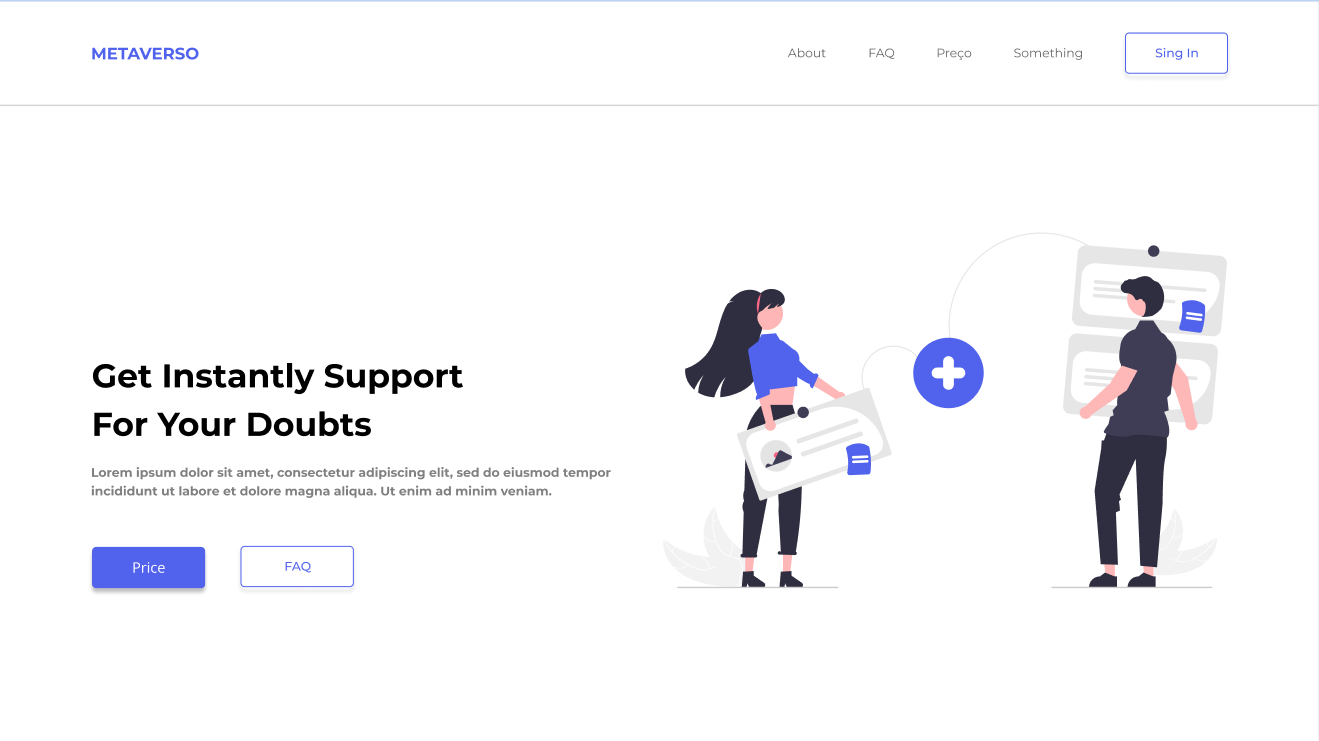
\includegraphics[width=1\textwidth]{image/about-section.png}
\end{frame}

\begin{frame}{Free FAQ} 
    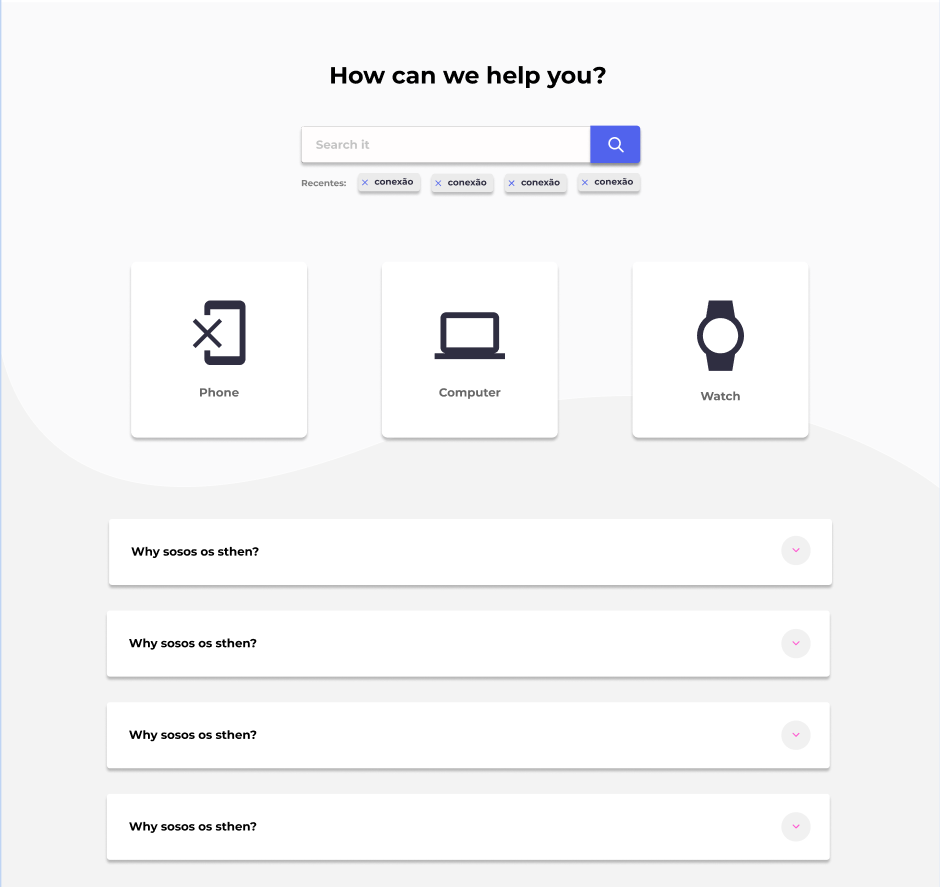
\includegraphics[width=1\textwidth]{image/faq.png}
\end{frame}

\begin{frame}{Planos} 
    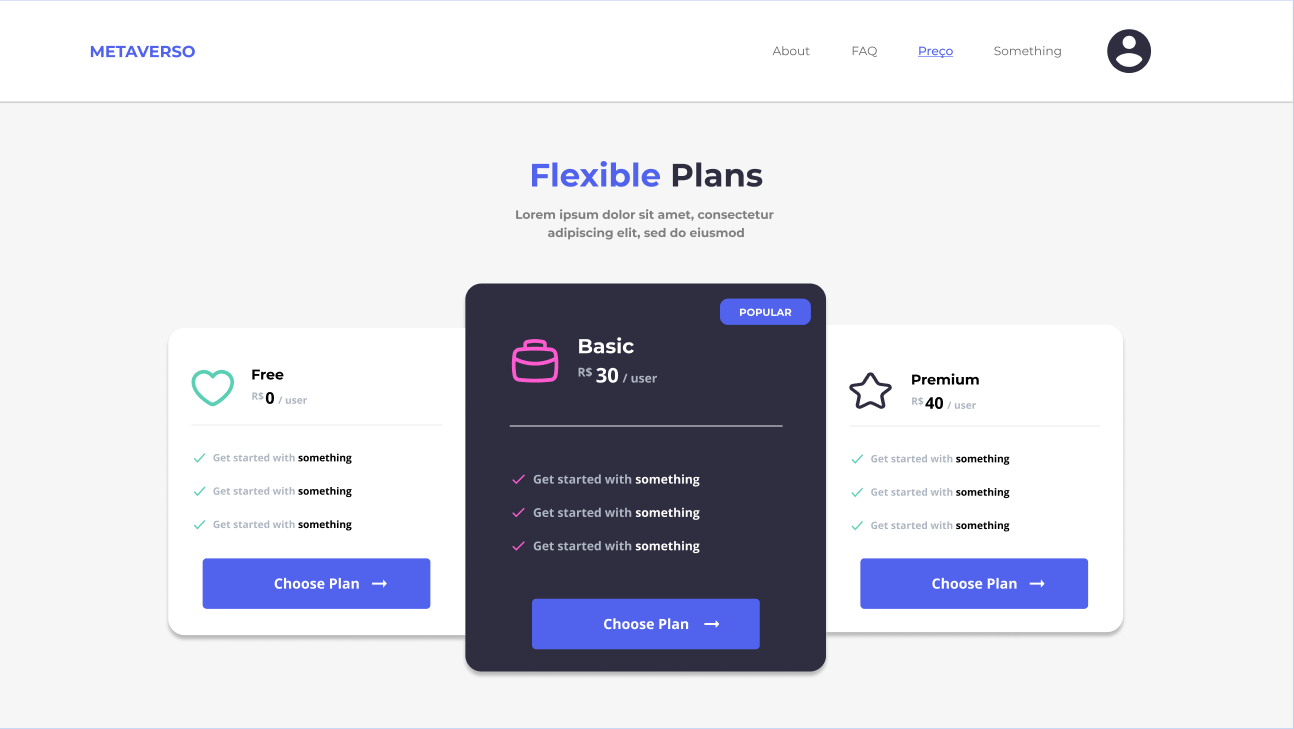
\includegraphics[width=1\textwidth]{image/plans.png}
\end{frame}

\begin{frame}{Log in} 
    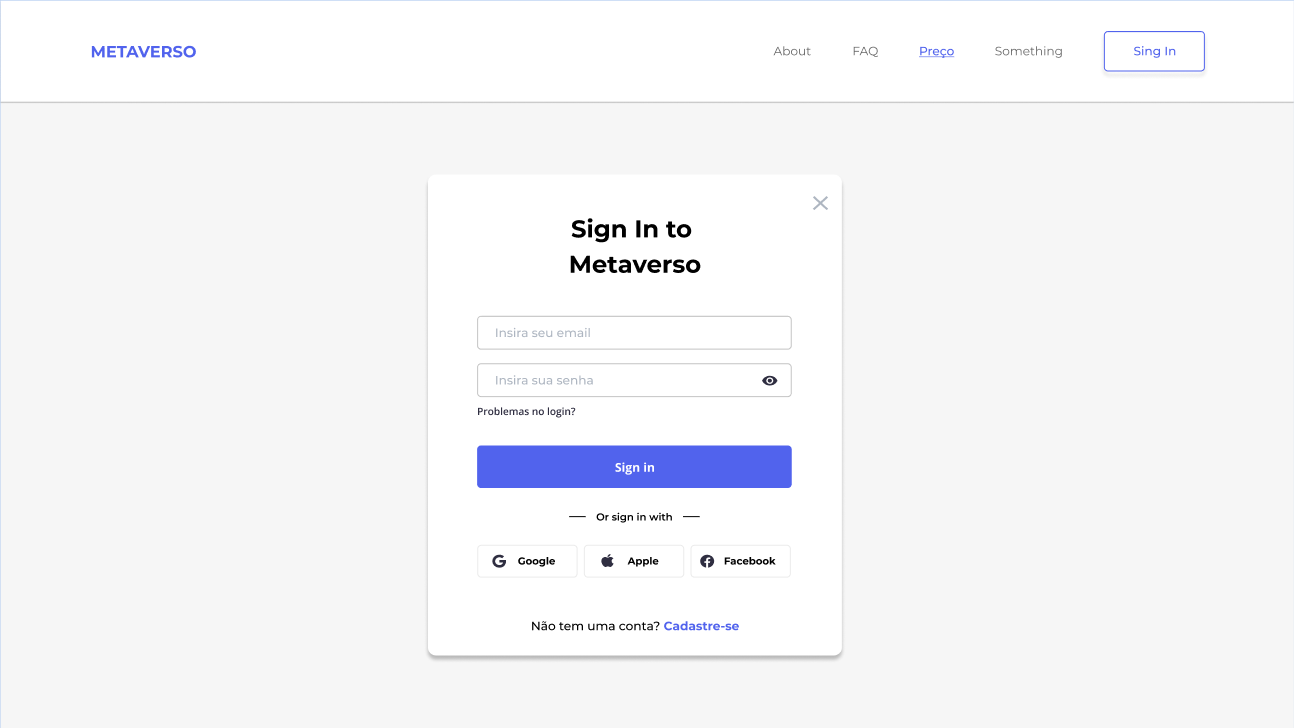
\includegraphics[width=1\textwidth]{image/login.png}
\end{frame}

\begin{frame}{Chamados} 
    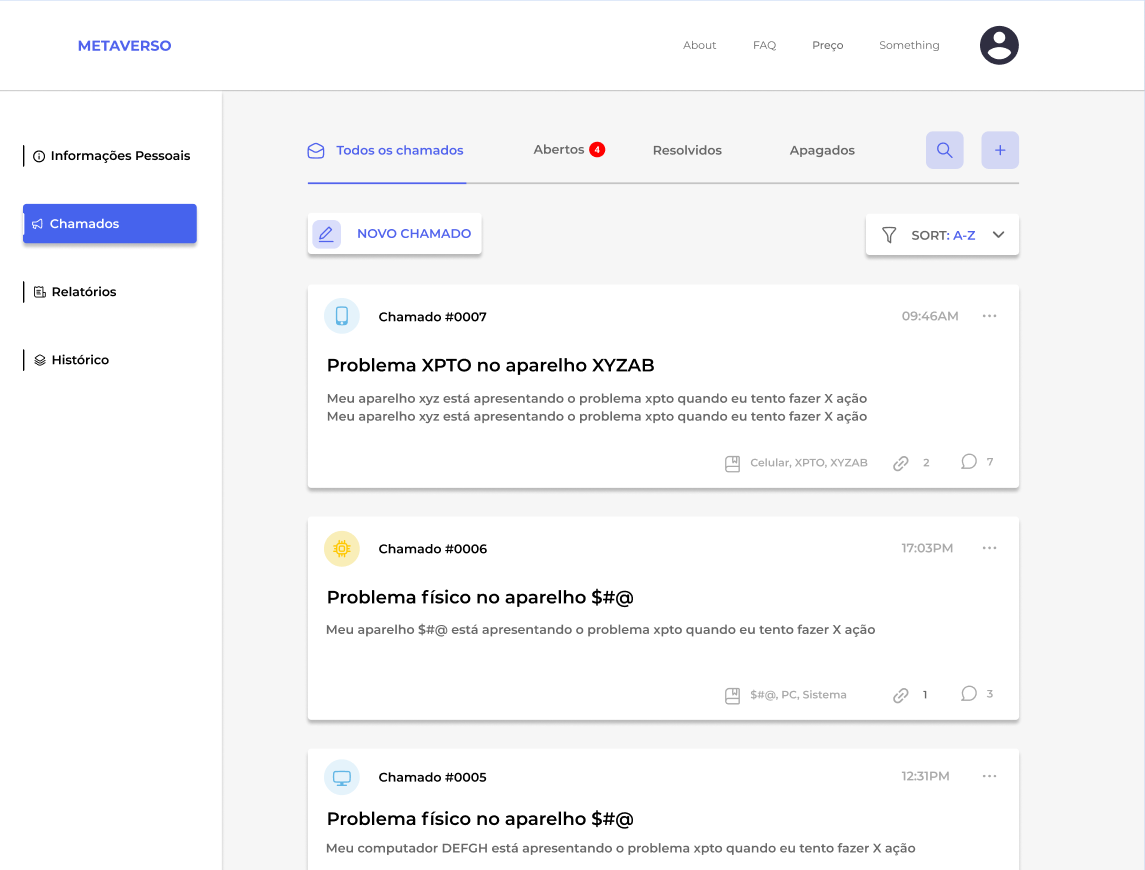
\includegraphics[width=0.95\textwidth]{image/dashboard-chamados.png}
\end{frame}

\begin{frame}{Novo Chamado} 
    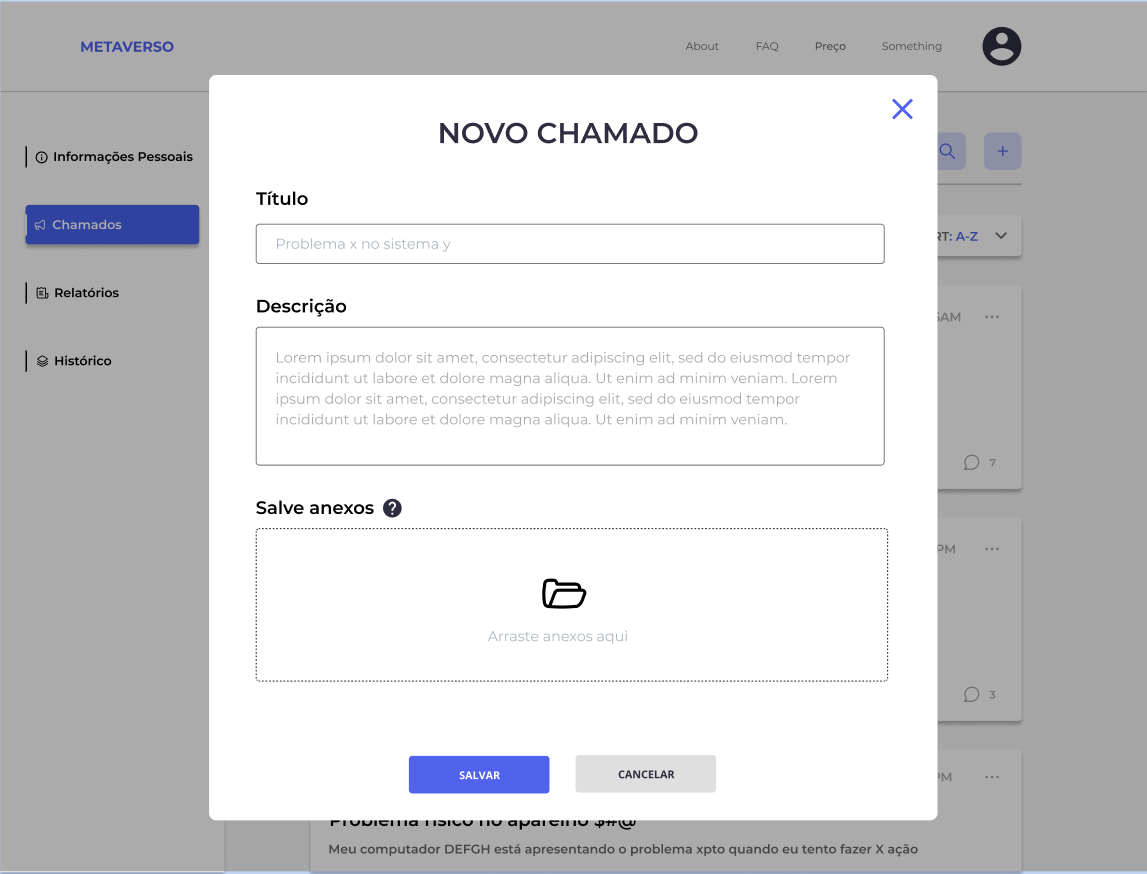
\includegraphics[width=0.95\textwidth]{image/novo-chamado.png}
\end{frame}

% * indica para não criar uma página de separação... e também não incluir na agenda
\section*{Dúvidas}

\newcommand{\urlApresentacao}{https://www.overleaf.com/project/62705e93d740b019b8d0c332}
\begin{frame}{Dúvidas} 

% Endereço da Apresentação e contatos com QR-Code para facilitar acesso
% Se for uma apresentação remota é importante colocar no CHAT da ferramenta os dados para facilitar mais ainda

% dependendo do público não é necessário colocar os contatos
% Esse layout de duas colunas foi escolhido no caso para facilitar a captura dos qr codes já que a camera pode vir pela direita ou esquerda sem muita dificuldade


    \begin{columns}[t]
    
        \begin{column}{0.45\textwidth}
            \begin{block}{Dúvidas}
                \begin{itemize}
                  \item Perguntas?
                \end{itemize}

                \begin{figure}
                    \centering
                    \qrcode{\urlApresentacao}
                    \caption*{Apresentação disponível em : \newline \url{\urlApresentacao}}
                \end{figure}

            \end{block}
        \end{column}
    
        % Exemplo de como gerar qr-code com email para contato....
    \end{columns}

\end{frame}


\end{document}